\documentclass[12pt]{article}
\usepackage[margin=1in]{geometry}
\usepackage{setspace}
\usepackage{graphicx}
\usepackage{booktabs}
\usepackage{amsmath}
\usepackage{natbib}
\usepackage{caption}
\usepackage[hidelinks]{hyperref}
\usepackage{microtype}
\bibliographystyle{plainnat}
\captionsetup{font=small,labelfont=bf}
\graphicspath{{../output/figures/}}

\title{\bf Prevention Without Proof}
\author{Scott Cunningham\\ \small Baylor University}
\date{\small Prepared for the European Commission, Joint Research Centre, Ispra \\ \small June 2026}

\begin{document}
\maketitle
\thispagestyle{empty}

\begin{abstract}
\noindent
For two decades the world's governments have answered suicide with national strategies, and for
two decades we have told ourselves they work. Testing the claim across Europe, I first show that the
standard difference-in-differences design is invalid here: adopting and non-adopting countries
differ sharply in the level of suicide and follow a significant pre-existing upward trend that
continues, unbroken, through adoption. Matching on that level path instead---augmented synthetic
control for each of the four adopting countries, and synthetic difference-in-differences by
cohort---yields small effects that permutation inference cannot distinguish from chance ($p$ between
$0.43$ and $0.79$). The strategies may work. These data cannot show it.
\end{abstract}

\vfill
\begin{center}
\small JEL: I18, I12, C23. \quad Keywords: suicide; synthetic control; difference-in-differences;
parallel trends; mental health policy.
\end{center}
\clearpage

\doublespacing
\setcounter{page}{1}

\section{Introduction}

Every forty seconds, somewhere on earth, a person decides that the rest of life is not worth the
rest of life. Confronted with more than seven hundred thousand such deaths a year, governments have
done what governments do: they have written strategies. Since the early 1990s the national
suicide-prevention strategy has spread from a Nordic experiment to an article of international
faith, and the World Health Organization now urges every member state to adopt one
\citep{who2014preventing,who2018strategies}. We have decided, collectively, that the document is the
cure. This paper asks whether the cross-national record can tell us if it is.

The question is harder than it looks, and most of this paper is about why. The natural research
design---compare suicide before and after adoption in adopting countries against the contemporaneous
change in non-adopters---is a difference-in-differences, and difference-in-differences rests on an
assumption that is simply false in this setting. Adopting countries are not faint copies of
non-adopters waiting to diverge; they are different places. They begin with markedly lower suicide
rates, an older population, and a different position in the business cycle, and---most damaging for
the design---they are already on a different \emph{trajectory}. A long panel shows a statistically
significant upward trend in adopters' suicide rates, relative to controls, that begins well before
any strategy is written and continues straight through the adoption date without a kink. A method
built on the premise of common trends cannot be trusted when the trends are demonstrably not common.

So I do not trust it, and Section~\ref{sec:did} explains in detail why no one should. When treated
and control units differ in both levels and trends, differencing does not remove the confound; it
extrapolates it. The appropriate response, set out by \citet{doudchenko2016balancing}, is to stop
differencing and start matching---to build, for each treated country, a weighted combination of
control countries that reproduces its pre-adoption \emph{path}, and then ask whether the treated
country departs from that synthetic match after adoption. That is the synthetic control method
\citep{abadie2010synthetic}, and Section~\ref{sec:scm} applies it, in its bias-corrected
ridge-augmented form \citep{benmichael2021augmented}, to each of the four European countries that
adopted a strategy with enough pre-adoption history to support the method.

The answer is the same for all four, and it is not the answer the literature expects. The synthetic
matches track the treated countries closely before adoption. After adoption the gaps are small and,
under permutation inference, ordinary: the post-to-pre fit ratios fall in the middle of the placebo
distribution, with $p$-values between $0.43$ and $0.79$. Synthetic difference-in-differences, fit
separately for each adoption cohort \citep{arkhangelsky2021synthetic}, gives the same verdict. The
estimates are not protective; they are not harmful; they are not distinguishable from zero.

I want to be precise about the claim, because it is easy to misread. I am not claiming that
suicide-prevention strategies fail. I am claiming that the cross-national observational record
cannot determine whether they succeed---that the treated and control countries are too different in
levels and trends for differencing to identify anything, and that when one uses the design suited to
that difference, no effect emerges from the noise. A policy can be both worth keeping and unproven.
What is not defensible is the laundering of a confounded association into a causal claim, which is
what the field has done. The contribution here is to show, carefully and with the right tools, how
little we actually know.

\section{A Policy Adopted Without Evidence}

The modern national strategy was born in Finland, which between 1986 and 1992 investigated every
suicide in the country and built a prevention program on what it learned. Norway and Sweden followed
in 1995, the United Kingdom in 2002, Ireland in 2005; by 2018 the WHO could count dozens of national
strategies and exhort the rest \citep{who2018strategies}. The diffusion was rapid and sincere. It
was also almost entirely uninformed by credible evidence, because the one widely cited evaluation,
\citet{matsubayashi2011effect}, compared adopters and non-adopters with a two-way fixed-effects
estimator---before the profession understood what that estimator does under staggered timing and
heterogeneous effects \citep{goodmanbacon2021did,dechaisemartin2020twoway}. Appendix~B shows, via a
Goodman-Bacon decomposition, that two-way fixed effects is not in fact the binding problem in these
data. The binding problem is more basic, and it afflicts every estimator that differences: the
groups are not comparable.

\section{Data}
\label{sec:data}

The outcome is the age-standardized suicide rate---deaths from intentional self-harm per hundred
thousand. From 1994 onward I use the figures Eurostat publishes for the European Union
\citep{eurostat_cod}. To give the design the long pre-adoption window that both the trend diagnostic
and the synthetic control require, I extend the series back to 1986 using the WHO Mortality Database
\citep{who_mdb}, chained to the Eurostat level by a country-specific multiplicative factor estimated
on the 1994--2010 overlap (Appendix~A; the two sources use different standard populations, so the
splice is a documented approximation). Treatment is the year a government adopted a stand-alone
national strategy \citep{who2018strategies,lewitzka2019national}. The balanced panel covers
seventeen countries from 1986 to 2010: four adopters (Norway and Sweden in 1995, the United Kingdom
in 2002, Ireland in 2005) and thirteen documented never-adopters, among them Italy, Spain, Belgium,
Austria, Switzerland, the Netherlands, and Portugal. Italy---the country in which these words are
read---never wrote the document, and stands throughout as the natural point of comparison.

\section{Why Difference-in-Differences Is the Wrong Design Here}
\label{sec:did}

\subsection{The estimand and what it requires}

The object of interest is the average effect of adoption on suicide in the countries that adopted.
Difference-in-differences recovers it only under parallel trends: absent treatment, adopters' suicide
rates would have moved in parallel with non-adopters'. Parallel trends is not a technical nicety to
be waved through. It is the whole identifying content of the design, and it is an assumption about
counterfactual \emph{trajectories}---which means the data can speak to its plausibility through the
pre-adoption period, even though it can never be verified after.

\subsection{The groups differ in levels}

Table~\ref{tab:balance} reports baseline (1994) means and the standardized difference between
adopters and never-adopters. \citet{imbens2015causal} call a covariate imbalanced when that
difference exceeds $0.25$ in absolute value; here every comparable covariate does. Adopters begin
with far \emph{lower} suicide ($-0.99$), higher unemployment ($+0.33$), an older population
($+0.63$ on the share over 65), and a lower median age. These are not the marginal imbalances that
covariate adjustment is designed to absorb; they are evidence that the treated and control groups are
different kinds of country.

\begin{table}[h]
\centering\small
\caption{Baseline (1994) balance, adopters vs.\ never-adopters. Standardized difference exceeding
$0.25$ in absolute value is ``imbalanced'' \citep{imbens2015causal}.}
\label{tab:balance}
\begin{tabular}{lcccc}
\toprule
Variable & Adopters & Never-adopters & Std.\ diff. & Imbalanced? \\
\midrule
Suicide rate (per 100k) & $12.13$ & $21.53$ & $-0.99$ & yes \\
Unemployment rate (\%) & $9.78$ & $8.18$ & $+0.33$ & yes \\
Share aged 65+ (\%) & $15.23$ & $13.95$ & $+0.63$ & yes \\
Median age (years) & $35.20$ & $36.24$ & $-0.42$ & yes \\
\bottomrule
\end{tabular}
\end{table}

\subsection{The groups differ in trends}

Differences in levels alone would not sink a difference-in-differences; differences in \emph{trends}
do. Figure~\ref{fig:didfails} plots the event study---each coefficient a long difference from the
year before adoption, the baseline against which both the post-treatment effects and the
parallel-trends assumption are defined. The pre-adoption coefficients are not scattered flatly around
zero. They rise. A weighted regression through them gives a slope of $+0.32$ suicides per hundred
thousand per year (\,$t = 3.4$, $p = 0.001$\,): adopters' suicide rates were climbing relative to
controls for a decade before any strategy existed. And the dashed line---that pre-trend, extrapolated
forward---runs straight through the post-adoption coefficients. There is no break at adoption. The
apparent ``effect'' is the continuation of a trend that predates the policy.

\begin{figure}[t]
\centering
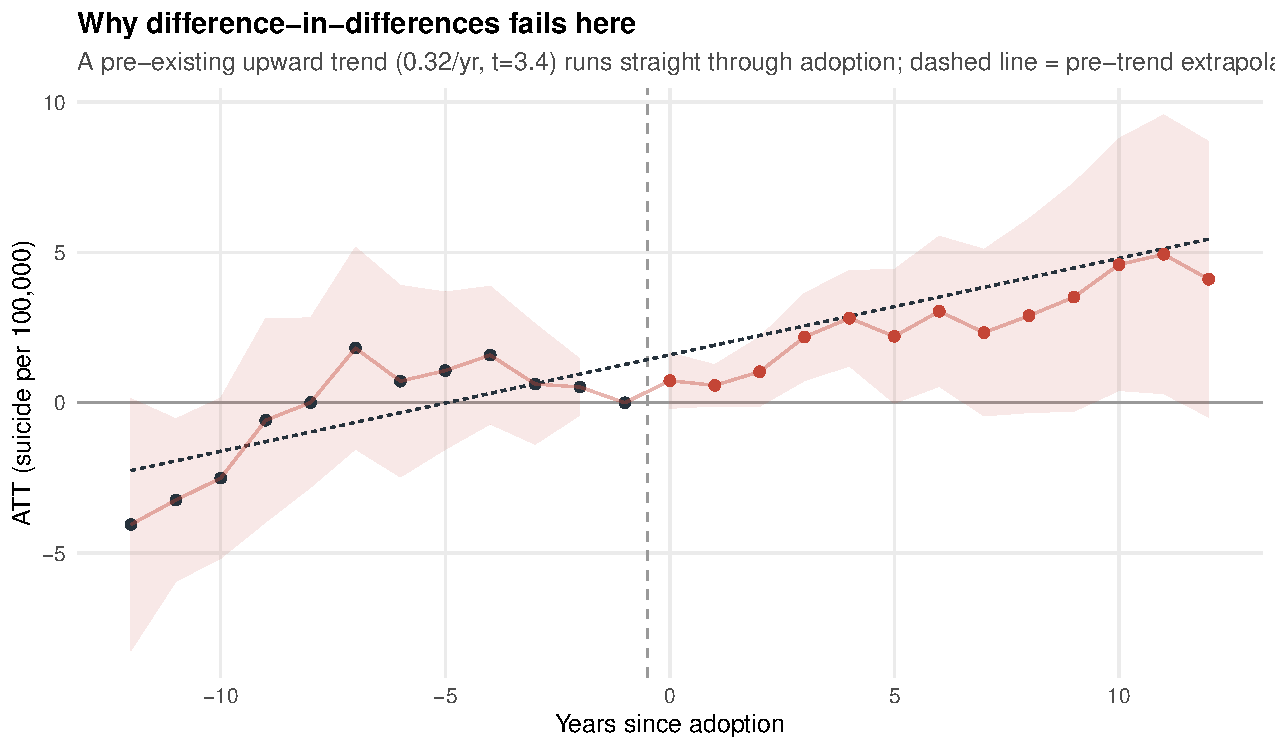
\includegraphics[width=0.86\textwidth]{fig_did_fails.pdf}
\caption{The pre-trend that invalidates differencing. Event study on the 1986--2010 panel (long
differences from the year before adoption). A significant upward trend ($+0.32$/year, $t=3.4$) runs
unbroken through the adoption date; the dashed line is the pre-trend extrapolated into the
post-period.}
\label{fig:didfails}
\end{figure}

\subsection{The implication: match, do not difference}

When treated and control units differ in both levels and trends, the difference-in-differences
estimate is not a treatment effect plus mean-zero noise; it is a treatment effect plus the
extrapolated trend gap, and the two cannot be separated.
\citet{doudchenko2016balancing} make the general point: differencing is the right tool only when the
untreated trajectory is a good counterfactual for the treated one, and when it is not, one should
instead reweight control units to reproduce the treated unit's pre-treatment path. This is the last
entry on the design checklist, and it is the one most often skipped---the instruction, when the
groups are this different, to \emph{stop differencing}. The rest of the paper follows it.

\section{Synthetic Control: Matching on the Level Path}
\label{sec:scm}

\subsection{Construction and augmentation}

For each adopting country I construct a synthetic control: a weighted average of the thirteen
never-adopters chosen to reproduce the adopter's suicide path over its full pre-adoption window
\citep{abadie2010synthetic}. Where the pre-adoption fit is imperfect, the simplex weights are
bias-corrected by the ridge augmentation of \citet{benmichael2021augmented}, which permits small
negative weights to close residual gaps. Norway and Sweden adopt in 1995 and so have nine
pre-adoption years in the extended panel; the United Kingdom has sixteen and Ireland nineteen.

\subsection{Fit and donor weights}

Figure~\ref{fig:scmfit} shows, for each country, the observed suicide path against its synthetic
match. The pre-adoption fit is close---pre-period root-mean-squared prediction errors of $0.7$
(Norway), $0.6$ (Sweden), $0.3$ (the United Kingdom), and $1.1$ (Ireland)---so the synthetic
controls are credible counterfactuals in a way the raw never-adopter average, with its different
level and trend, is not. Figure~\ref{fig:scmweights} shows where the weight falls, before and after
augmentation: pure synthetic control places non-negative weight on a handful of donors; ridge
augmentation adjusts those weights, and where the raw fit was poor (Ireland) it moves them
appreciably and allows a few to go negative, the signature of the bias correction at work.

\begin{figure}[t]
\centering
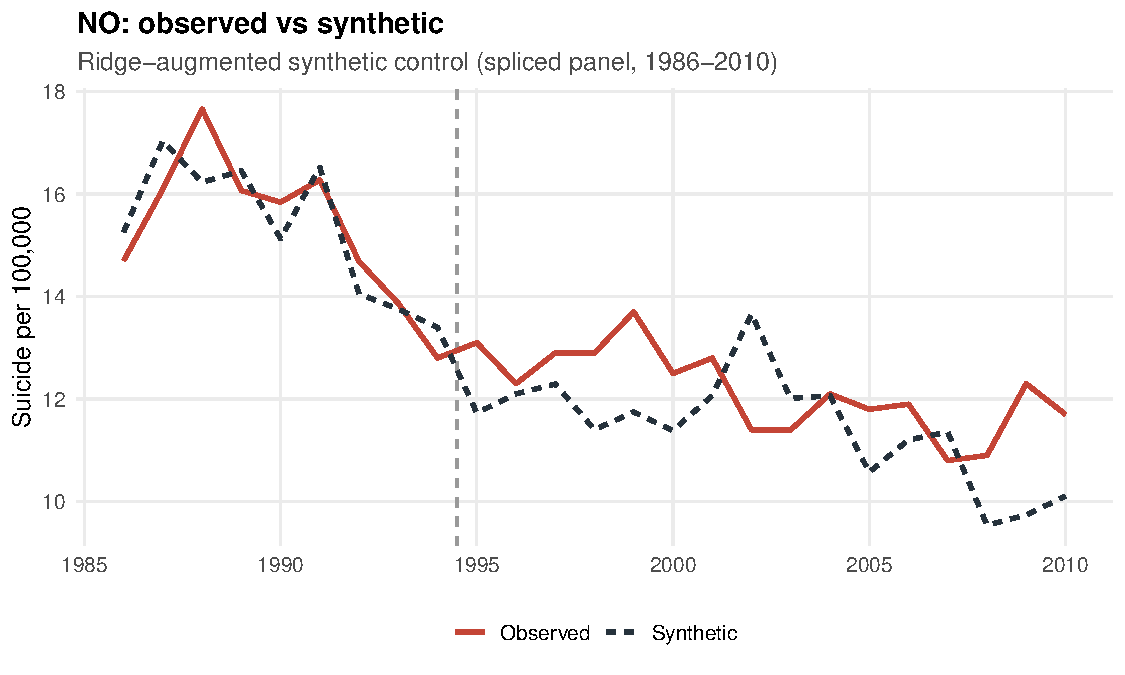
\includegraphics[width=0.49\textwidth]{fig_scm_fit_NO.pdf}\hfill
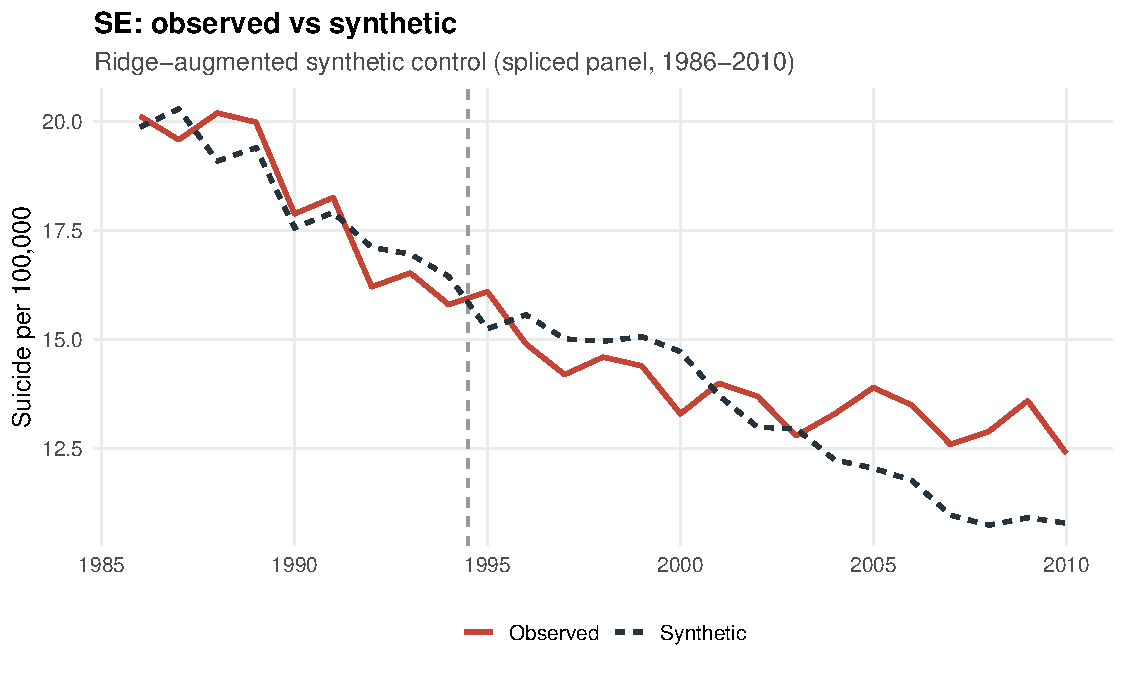
\includegraphics[width=0.49\textwidth]{fig_scm_fit_SE.pdf}\\[2pt]
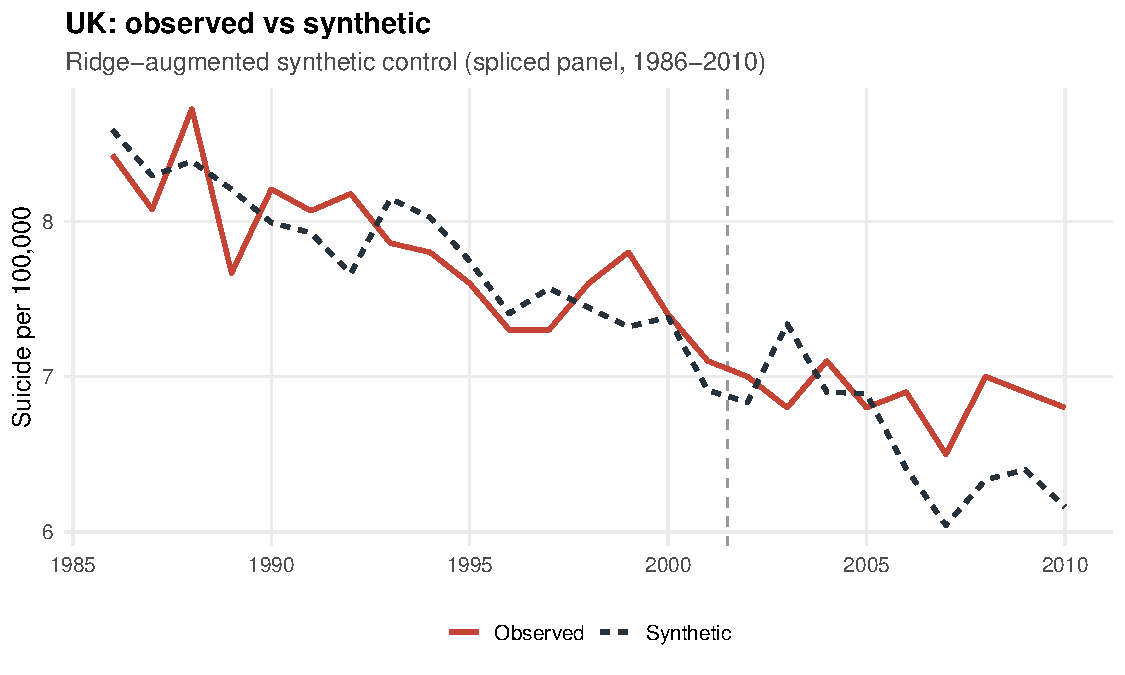
\includegraphics[width=0.49\textwidth]{fig_scm_fit_UK.pdf}\hfill
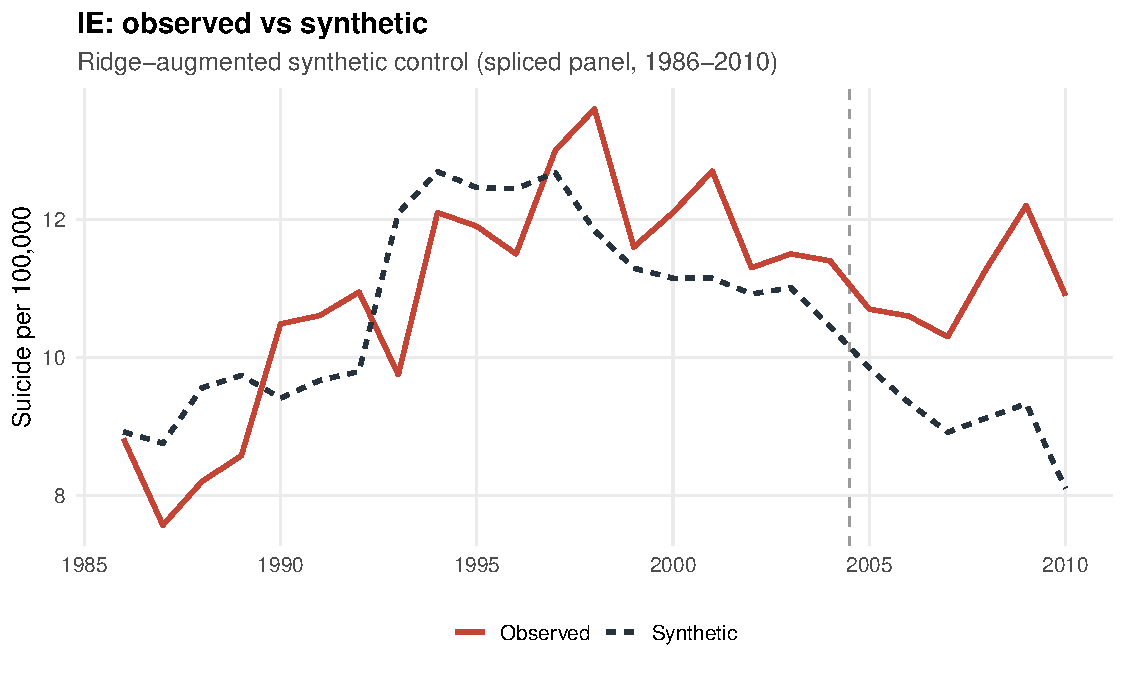
\includegraphics[width=0.49\textwidth]{fig_scm_fit_IE.pdf}
\caption{Observed (solid) vs.\ synthetic (dashed) suicide rate for each adopter. Vertical line marks
adoption. The synthetic controls track the pre-adoption path closely.}
\label{fig:scmfit}
\end{figure}

\begin{figure}[t]
\centering
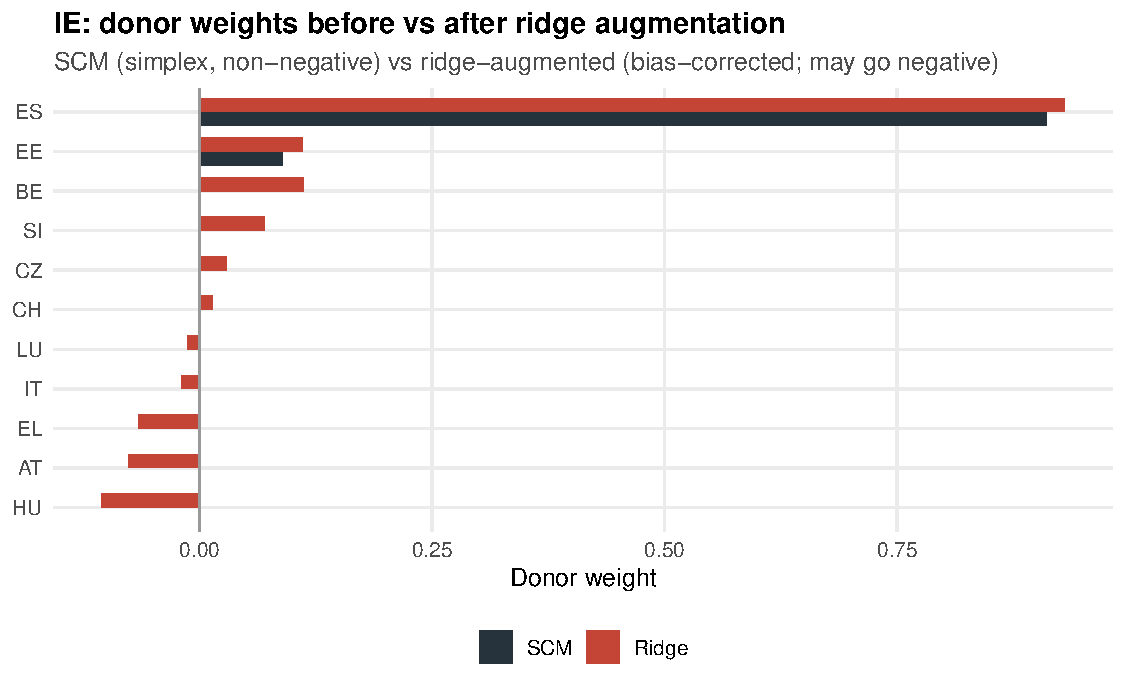
\includegraphics[width=0.49\textwidth]{fig_scm_weights_IE.pdf}\hfill
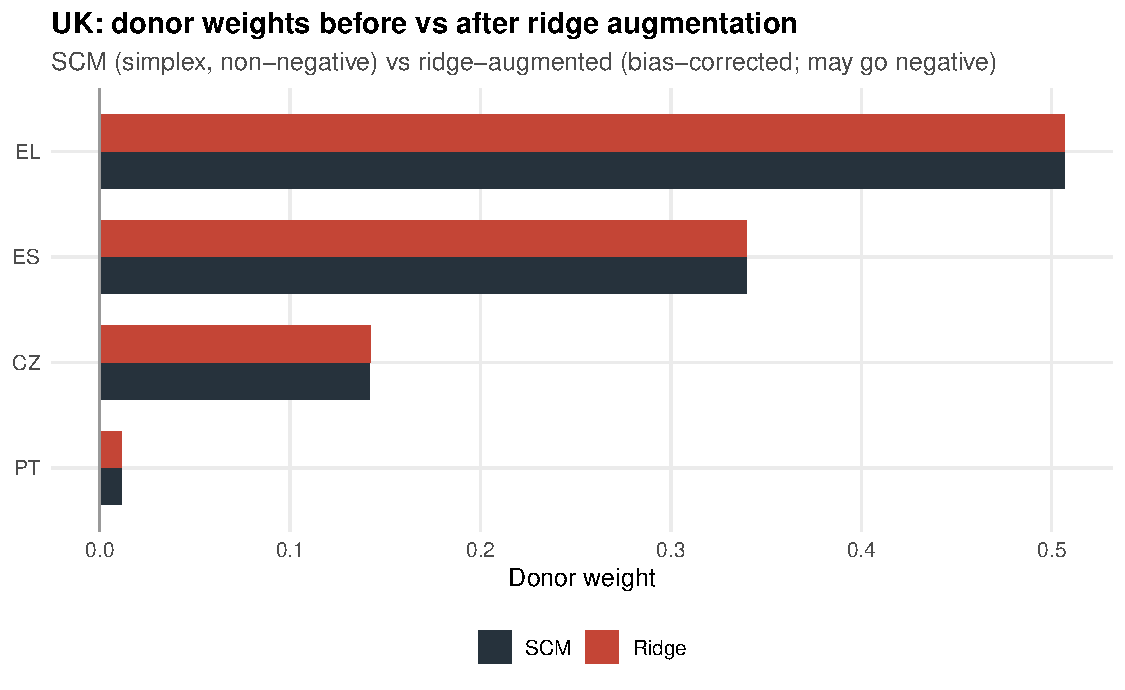
\includegraphics[width=0.49\textwidth]{fig_scm_weights_UK.pdf}
\caption{Donor weights before (SCM, non-negative simplex) and after (ridge-augmented) bias
correction, for Ireland (poor raw fit, large correction) and the United Kingdom (excellent raw fit,
negligible correction).}
\label{fig:scmweights}
\end{figure}

\subsection{Effects and permutation inference}

After adoption the treated countries drift above their synthetic matches, but modestly: average
post-adoption gaps of $+0.72$ (Norway), $+0.65$ (Sweden), $+0.28$ (the United Kingdom), and $+1.89$
(Ireland) suicides per hundred thousand---all of the same, wrong, sign as the literature's protective
claim. To gauge whether these are signal, I use permutation inference \citep{abadie2010synthetic}:
reassign treatment to each never-adopter in turn, compute its post-to-pre fit ratio, and rank the
treated country against that placebo distribution. The treated countries are unremarkable
(Figure~\ref{fig:scmperm}): permutation $p$-values of $0.71$ (Norway), $0.71$ (Sweden), $0.79$ (the
United Kingdom), and $0.43$ (Ireland). A randomly chosen never-adopter is about as likely to show a
post-adoption gap this large as the countries that actually adopted.

\begin{figure}[t]
\centering
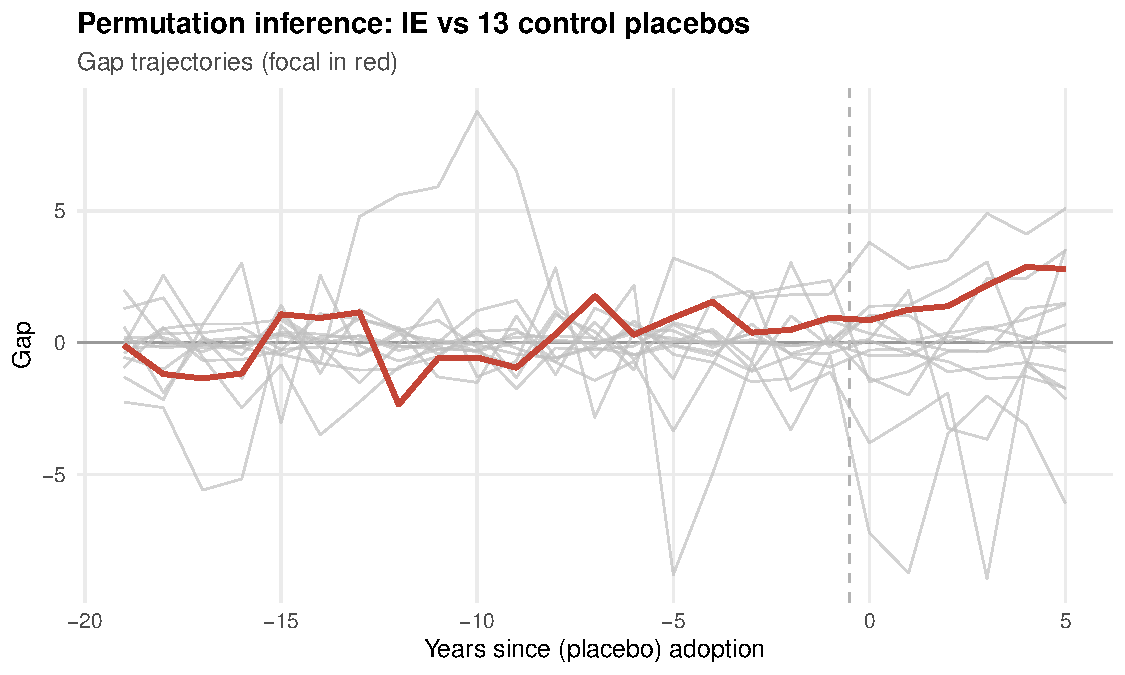
\includegraphics[width=0.49\textwidth]{fig_scm_spaghetti_IE.pdf}\hfill
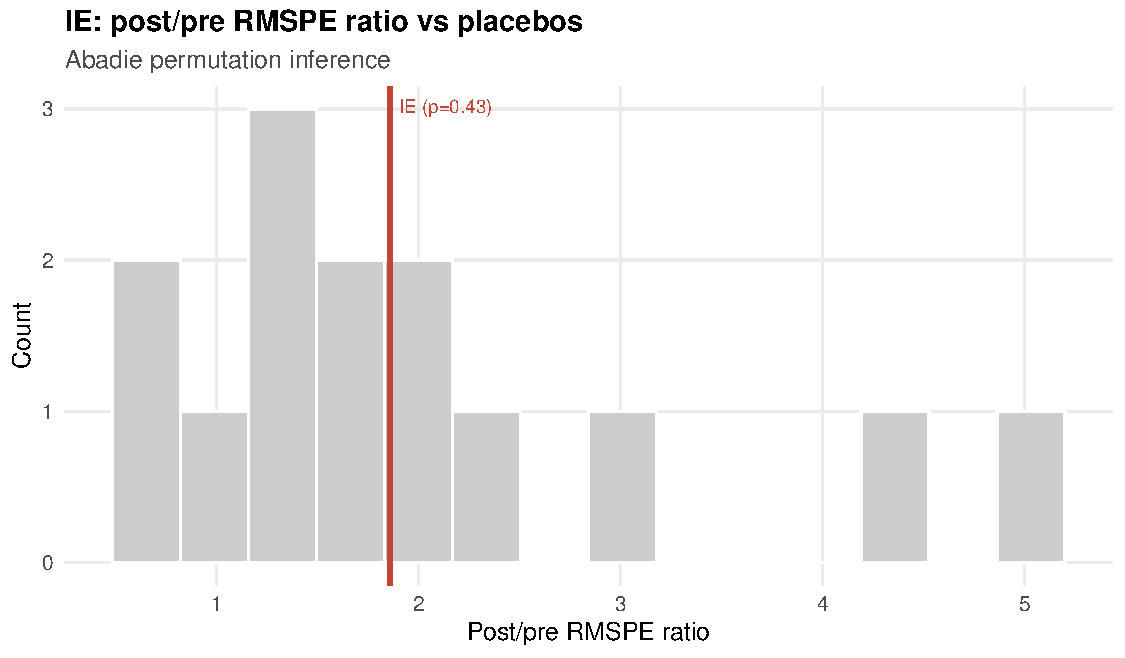
\includegraphics[width=0.49\textwidth]{fig_scm_rmspe_IE.pdf}
\caption{Permutation inference, Ireland. Left: gap trajectories for Ireland (red) against placebo
gaps from each never-adopter (grey). Right: Ireland's post/pre RMSPE ratio against the placebo
distribution ($p=0.43$).}
\label{fig:scmperm}
\end{figure}

\subsection{Synthetic difference-in-differences by cohort}

Finally I estimate, for each adoption cohort, the synthetic difference-in-differences of
\citet{arkhangelsky2021synthetic}, which reweights both control units and pre-periods to balance the
treated cohort before differencing---a hybrid that inherits synthetic control's robustness to the
level-and-trend gap. The cohort estimates are $+0.80$ (1995, Norway/Sweden), $+1.24$ (2002, the
United Kingdom), and $+0.74$ (2005, Ireland) suicides per hundred thousand, each with a standard
error larger than the estimate. The verdict does not move.

\section{What the Evidence Supports}

Three methods, applied to four countries and three cohorts, agree. The augmented synthetic controls,
the permutation tests, and the cohort-level synthetic difference-in-differences all return small,
wrong-signed, statistically ordinary differences. Set against the contaminated
difference-in-differences of Section~\ref{sec:did}, which cannot be interpreted at all, the picture
is consistent and sobering: the cross-national record contains no evidence that national
suicide-prevention strategies reduced suicide, and no power to rule out effects of either sign of a
size that would matter. This is not a null result in the comfortable sense of a precisely estimated
zero. It is the harder kind---an honest admission that the design space available to us, even used
correctly, cannot answer the question.

\section{Conclusion}

It is tempting, having shown that a famous claim does not survive scrutiny, to feel that something
has been settled. Very little has. The world's suicides are not reduced by a confidence interval, and
a country deciding tomorrow whether to write a strategy gains nothing from being told that the last
twenty years of evidence were thinner than advertised---unless that knowledge changes what it does
next. It should change two things. It should change our confidence: a policy can be worth keeping and
still unproven, and honesty requires holding both at once rather than citing a single discredited
comparison as if it closed the matter. And it should change how we invest in knowing. We adopted a
continent's worth of strategies without once building the variation---a staggered randomization, a
phased regional rollout with administrative mortality data, a pre-registered evaluation---that would
let us learn whether they work. If the European Commission wishes to know whether its mental-health
investments save lives, and it should, the evaluation must be designed before the policy is deployed,
below the level of the nation, with the counterfactual built in rather than reconstructed afterward
from a panel too small and too different to bear it. Until then we are governing mortality on faith,
and the first honest step is to say so.

\clearpage
\appendix
\singlespacing

\section{Appendix A: Data and the WHO--Eurostat Splice}

The outcome from 1994 is Eurostat's age-standardized suicide rate (table \texttt{hlth\_cd\_asdr},
ICD-10 X60--X84 and Y87.0, European Standard Population) \citep{eurostat_cod}. To 1986 I prepend the
WHO Mortality Database age-standardized rate \citep{who_mdb}, which uses the WHO World Standard
Population and therefore sits at a different level. Because the Eurostat-to-WHO ratio is stable within
country across the overlap (1994--2010), I chain multiplicatively: for each country I scale the
pre-1994 WHO values by the mean overlap ratio (estimated factors range from $1.05$ for Ireland to
$1.49$ for Portugal), placing them on the Eurostat scale. The spliced series is continuous across the
1993--1994 join. Germany is excluded because the WHO database has no unified pre-1990 German series;
the balanced panel is the seventeen countries with complete coverage 1986--2010. Treatment dates
follow the WHO 2018 inventory and \citet{lewitzka2019national}. The splice is an approximation and is
flagged as such; the results are robust to beginning the panel in 1990 (no splice for the 1995
cohort's first years) at the cost of shorter pre-windows.

\section{Appendix B: This Is Not a Two-Way-Fixed-Effects Artifact}

One might suspect the whole exercise reflects the known pathology of two-way fixed effects under
staggered timing \citep{goodmanbacon2021did}. It does not. The static two-way fixed-effects
regression returns a coefficient of $3.11$, and the Goodman-Bacon decomposition
(Table~\ref{tab:bacon}) reconstructs it exactly as a weighted average of its $2\times2$ components.
The ``forbidden'' comparisons that use already-treated countries as controls carry only about three
percent of the weight, because the never-treated pool is large; the clean treated-versus-untreated
comparisons carry the rest. Two-way fixed effects therefore sits beside the heterogeneity-robust
difference-in-differences estimate, and both are contaminated for the same reason---non-comparable
groups---not by negative weighting. The estimator is not the problem; the design is.

\begin{table}[h]
\centering\small
\caption{Goodman-Bacon decomposition of the two-way fixed-effects estimate}
\label{tab:bacon}
\begin{tabular}{lccc}
\toprule
$2\times2$ comparison & Weight & Avg.\ estimate & Contribution \\
\midrule
Treated vs.\ untreated & $0.864$ & $3.57$ & $3.085$ \\
Later vs.\ earlier treated & $0.112$ & $0.29$ & $0.032$ \\
Earlier vs.\ later treated & $0.025$ & $-0.22$ & $-0.005$ \\
\midrule
Reconstructed two-way fixed effects & $1.000$ & & $3.112$ \\
\bottomrule
\end{tabular}
\end{table}

\paragraph{Reproducibility.} Every estimate was computed in R (\texttt{did}, \texttt{augsynth},
\texttt{synthdid}, \texttt{fixest}, \texttt{bacondecomp}); the difference-in-differences results were
independently replicated in Python (\texttt{differences}) and Stata (\texttt{csdid}), with identical
samples and means and matching point estimates. The replication archive accompanies the paper.

\clearpage
\section{Appendix C: Full Synthetic-Control Diagnostics, All Four Adopters}

For completeness, the four diagnostics of Section~\ref{sec:scm}---observed-versus-synthetic fit, the
gap event study, donor weights before and after ridge augmentation, and permutation inference---are
shown here for each adopting country in turn. The pattern is uniform: close pre-adoption fit, a
modest and wrong-signed post-adoption gap, and a permutation rank that places the treated country in
the body of the placebo distribution rather than its tail.

\paragraph{Norway (adopted 1995; nine pre-periods; permutation $p=0.71$).}
\begin{figure}[h]
\centering
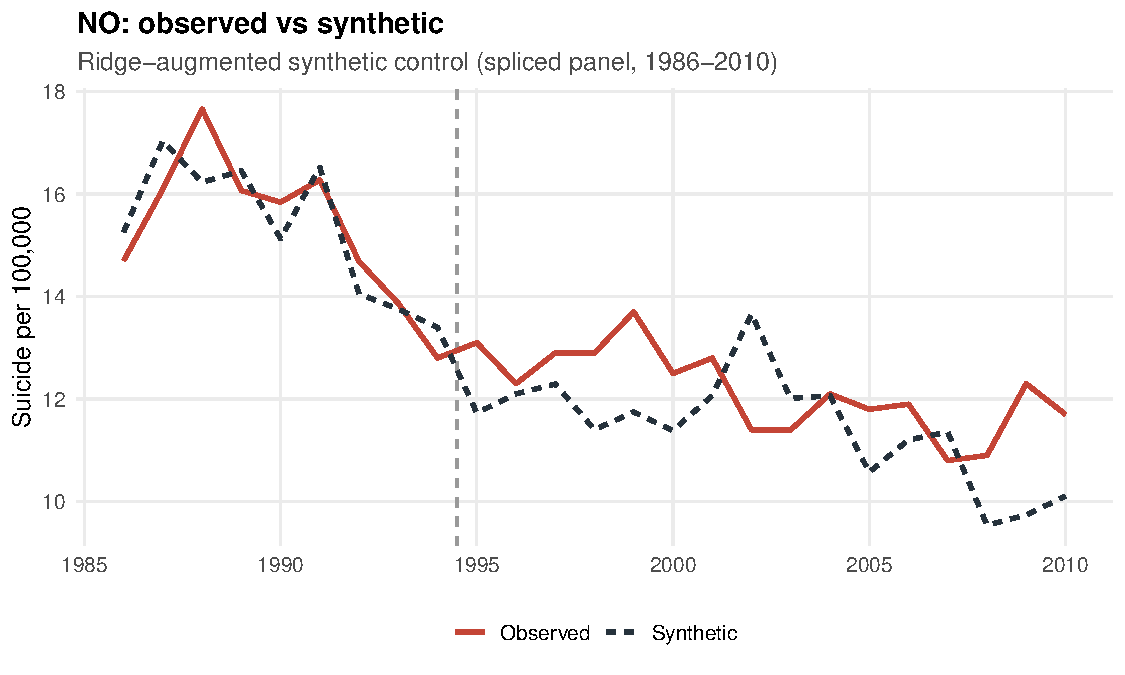
\includegraphics[width=0.49\textwidth]{fig_scm_fit_NO.pdf}\hfill
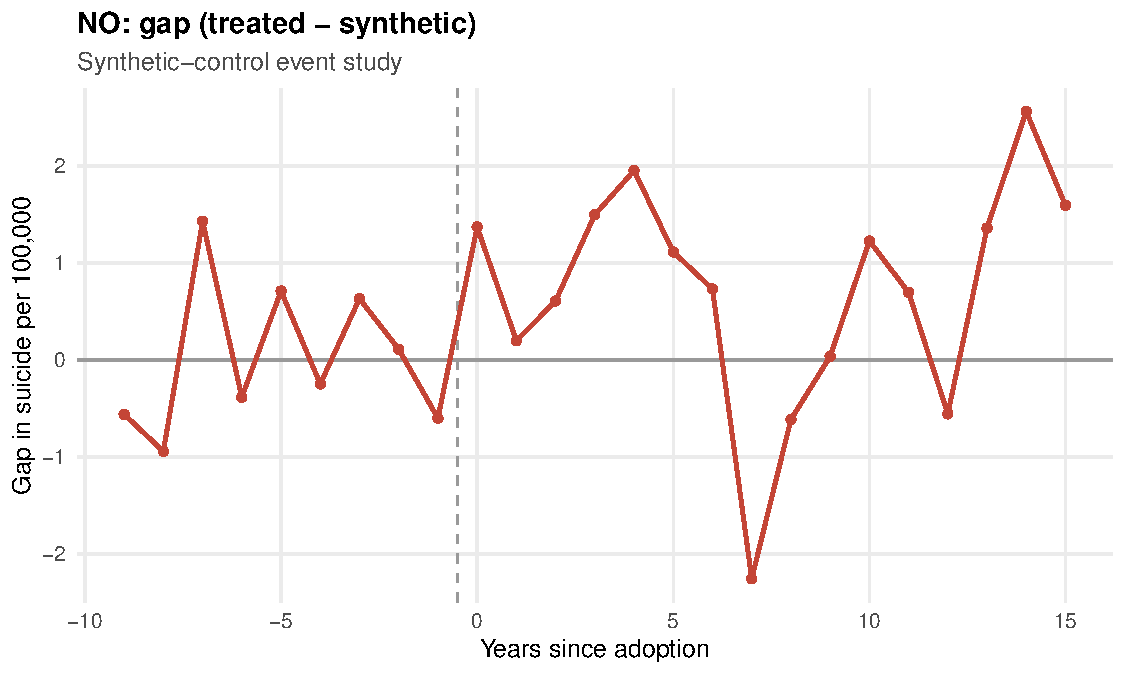
\includegraphics[width=0.49\textwidth]{fig_scm_gap_NO.pdf}\\[2pt]
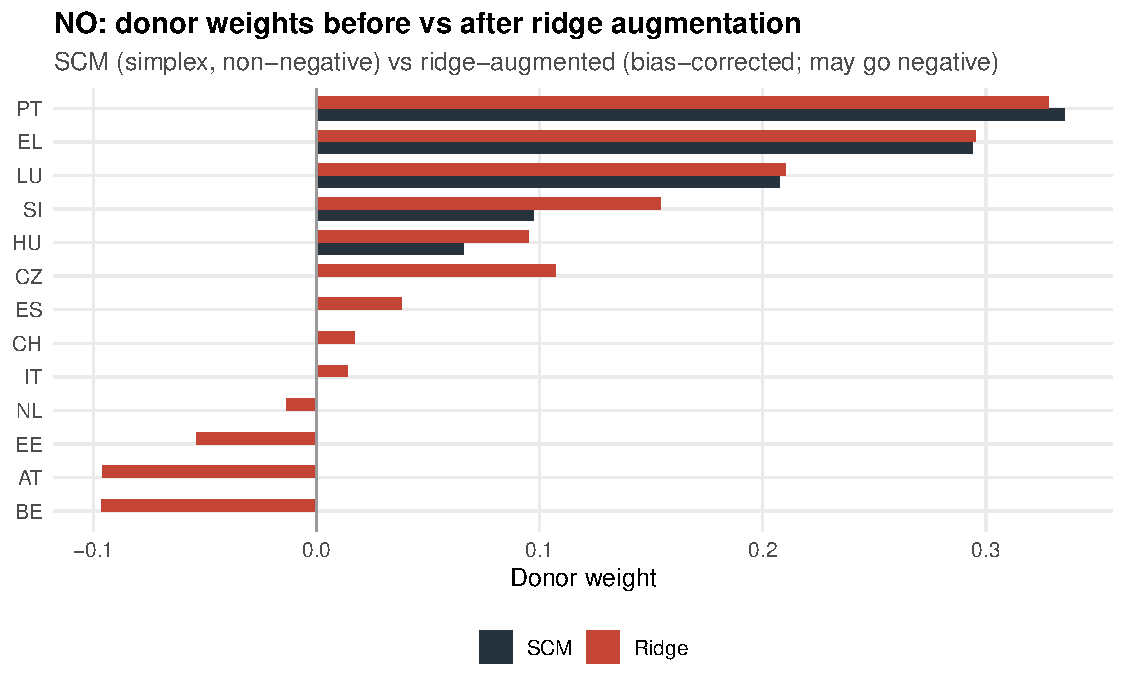
\includegraphics[width=0.49\textwidth]{fig_scm_weights_NO.pdf}\hfill
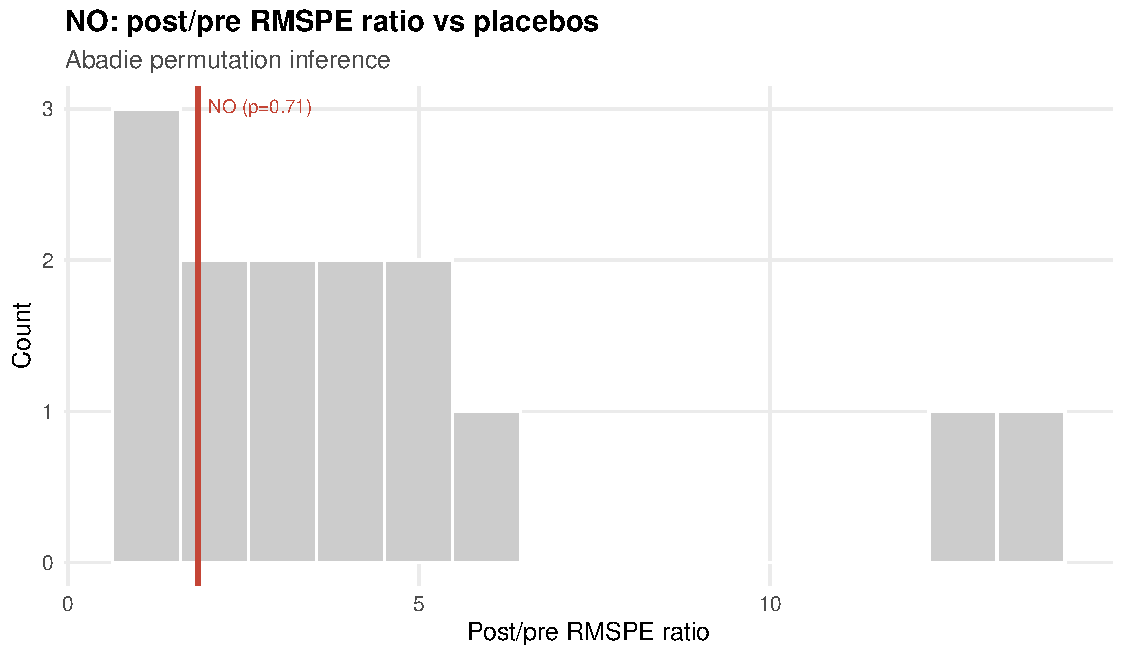
\includegraphics[width=0.49\textwidth]{fig_scm_rmspe_NO.pdf}
\caption{Norway. Fit, gap, donor weights (before/after ridge), and permutation.}
\end{figure}

\paragraph{Sweden (adopted 1995; nine pre-periods; permutation $p=0.71$).}
\begin{figure}[h]
\centering
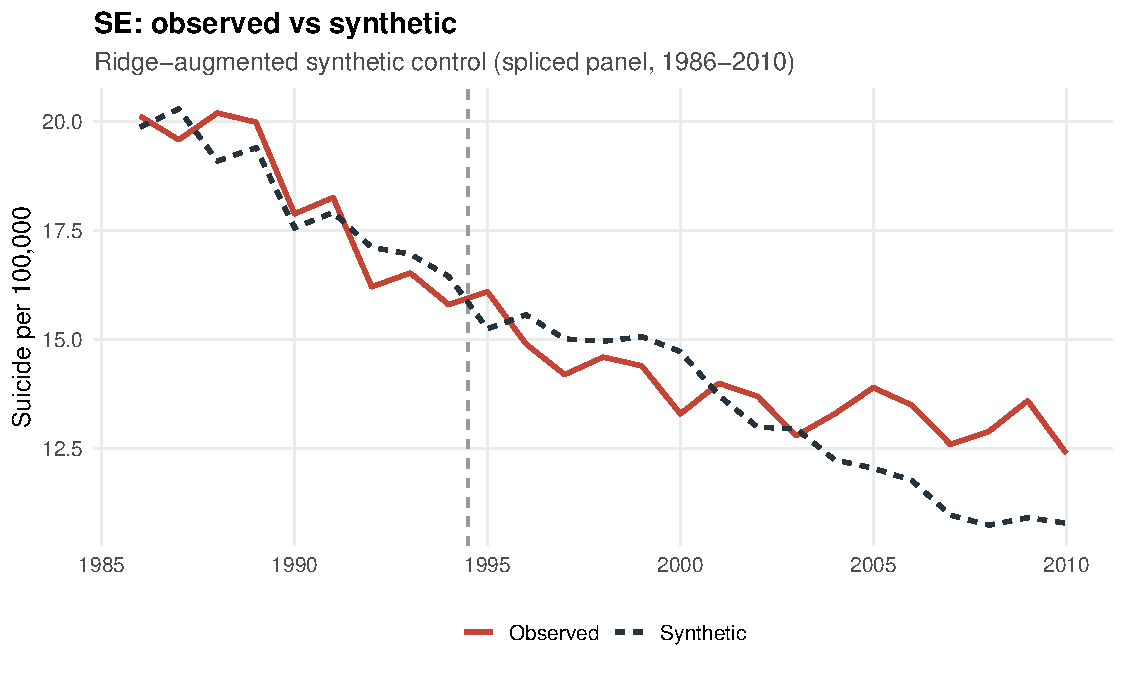
\includegraphics[width=0.49\textwidth]{fig_scm_fit_SE.pdf}\hfill
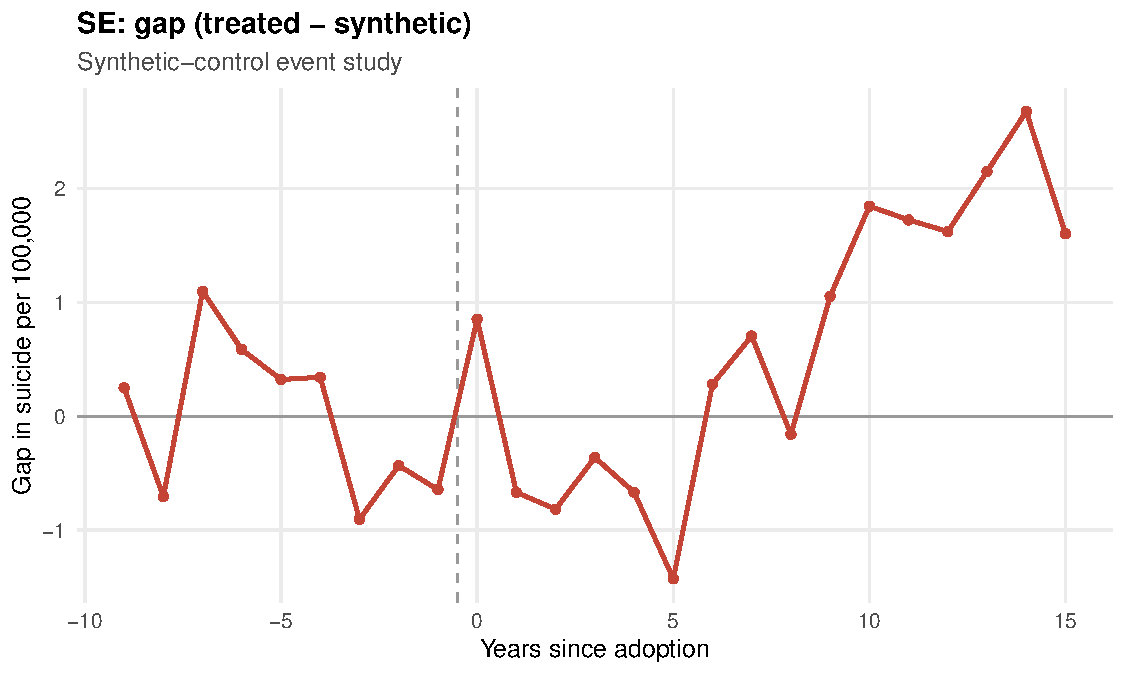
\includegraphics[width=0.49\textwidth]{fig_scm_gap_SE.pdf}\\[2pt]
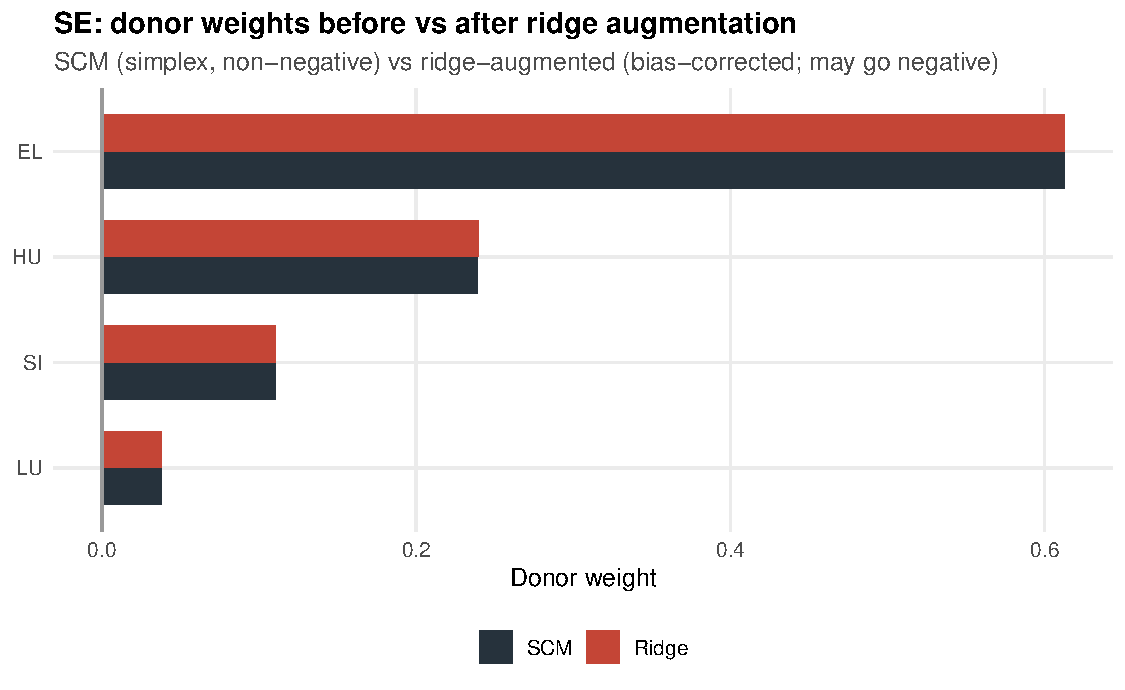
\includegraphics[width=0.49\textwidth]{fig_scm_weights_SE.pdf}\hfill
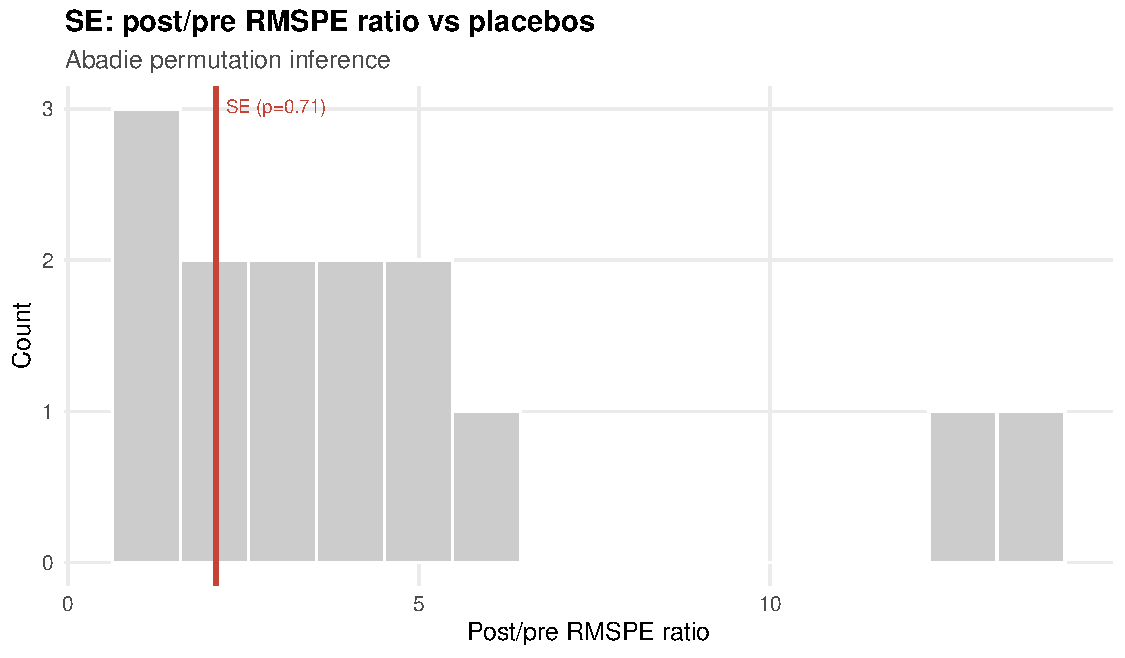
\includegraphics[width=0.49\textwidth]{fig_scm_rmspe_SE.pdf}
\caption{Sweden. Fit, gap, donor weights (before/after ridge), and permutation.}
\end{figure}

\clearpage
\paragraph{United Kingdom (adopted 2002; sixteen pre-periods; permutation $p=0.79$).}
\begin{figure}[h]
\centering
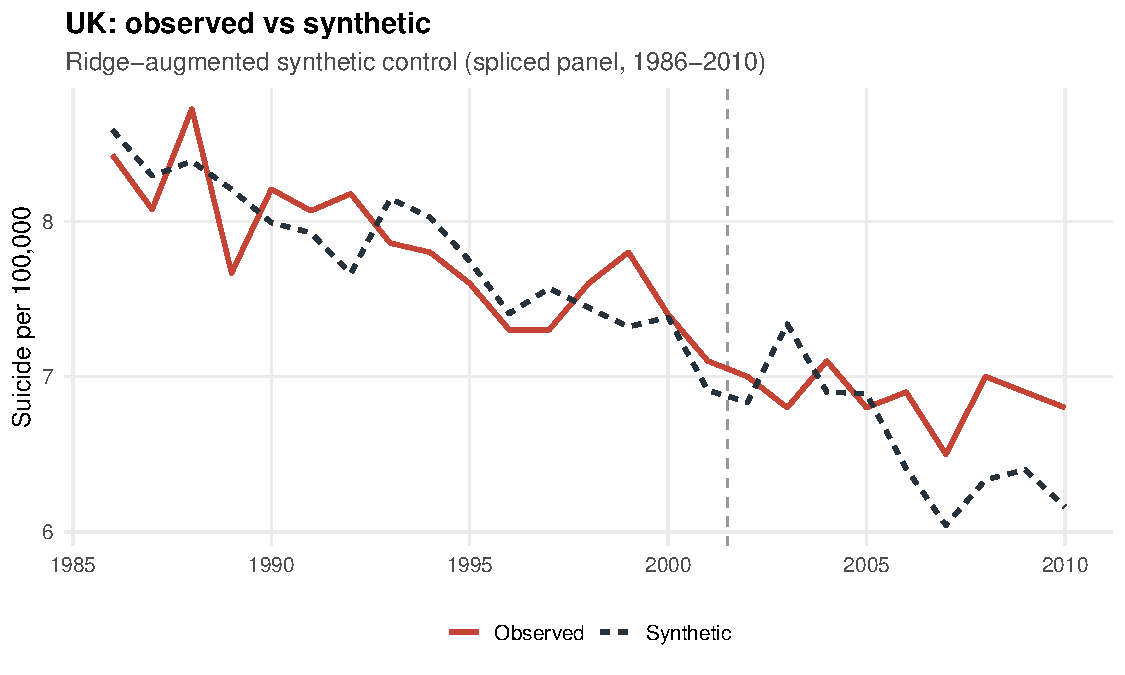
\includegraphics[width=0.49\textwidth]{fig_scm_fit_UK.pdf}\hfill
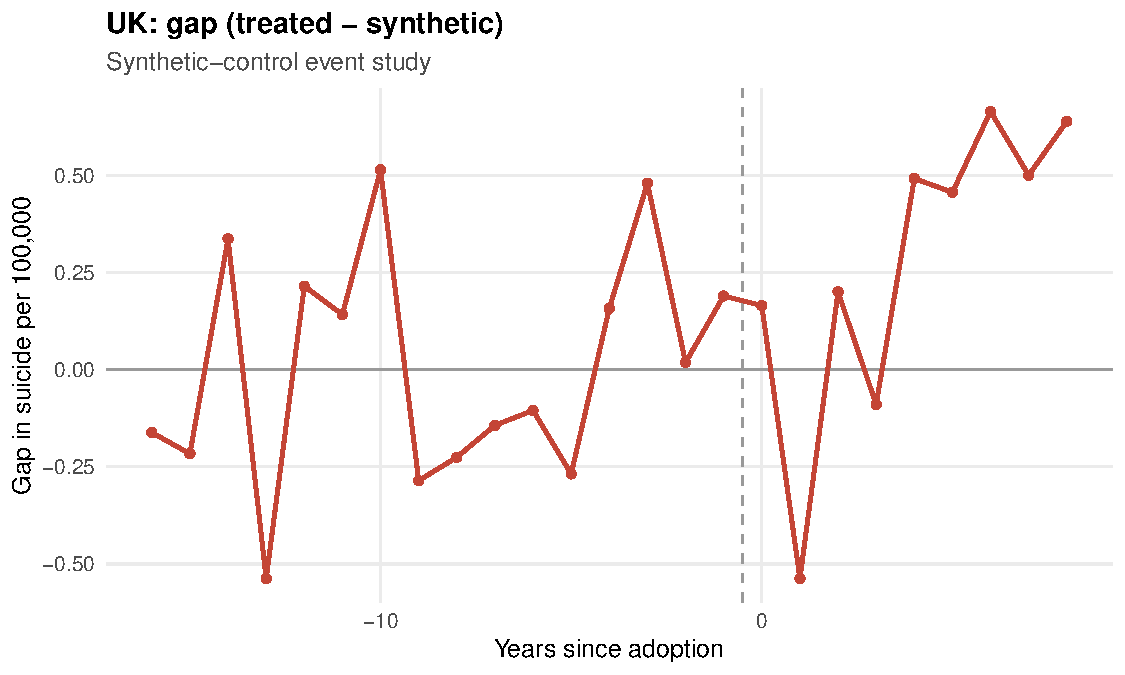
\includegraphics[width=0.49\textwidth]{fig_scm_gap_UK.pdf}\\[2pt]
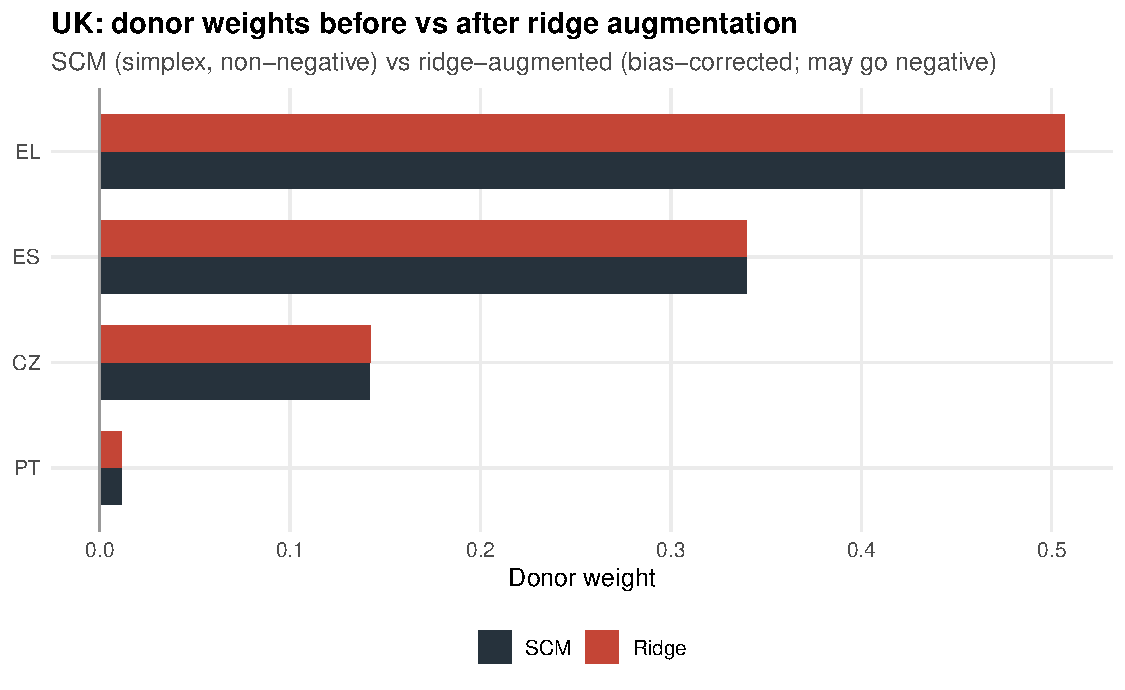
\includegraphics[width=0.49\textwidth]{fig_scm_weights_UK.pdf}\hfill
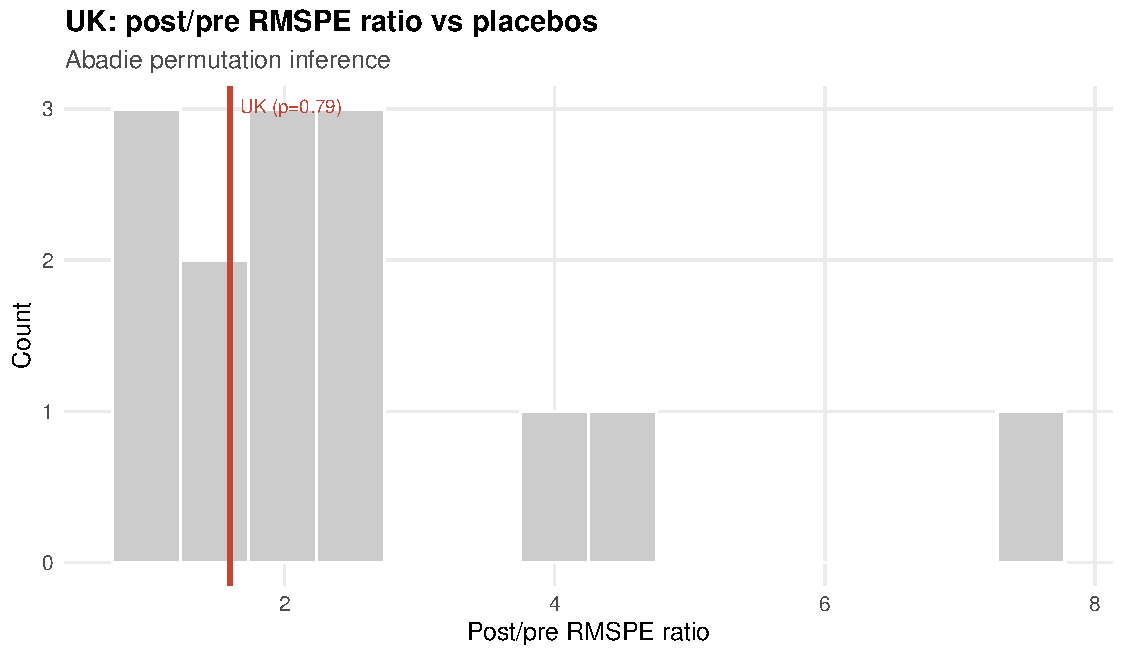
\includegraphics[width=0.49\textwidth]{fig_scm_rmspe_UK.pdf}
\caption{United Kingdom. Fit, gap, donor weights (before/after ridge), and permutation.}
\end{figure}

\paragraph{Ireland (adopted 2005; nineteen pre-periods; permutation $p=0.43$).}
\begin{figure}[h]
\centering
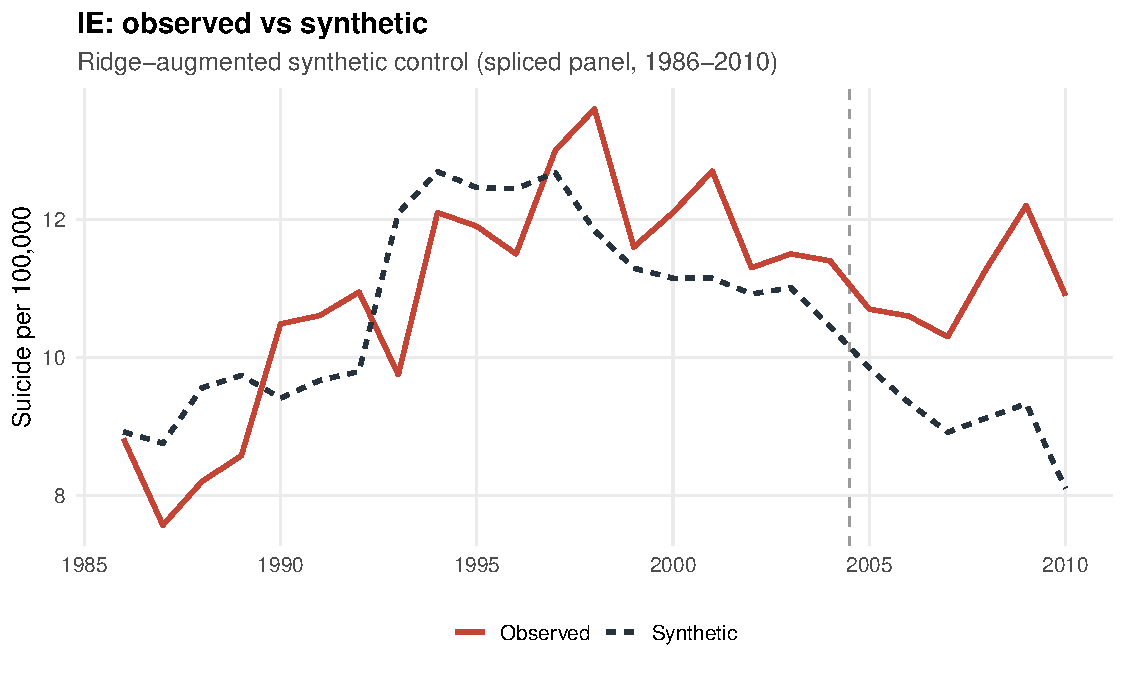
\includegraphics[width=0.49\textwidth]{fig_scm_fit_IE.pdf}\hfill
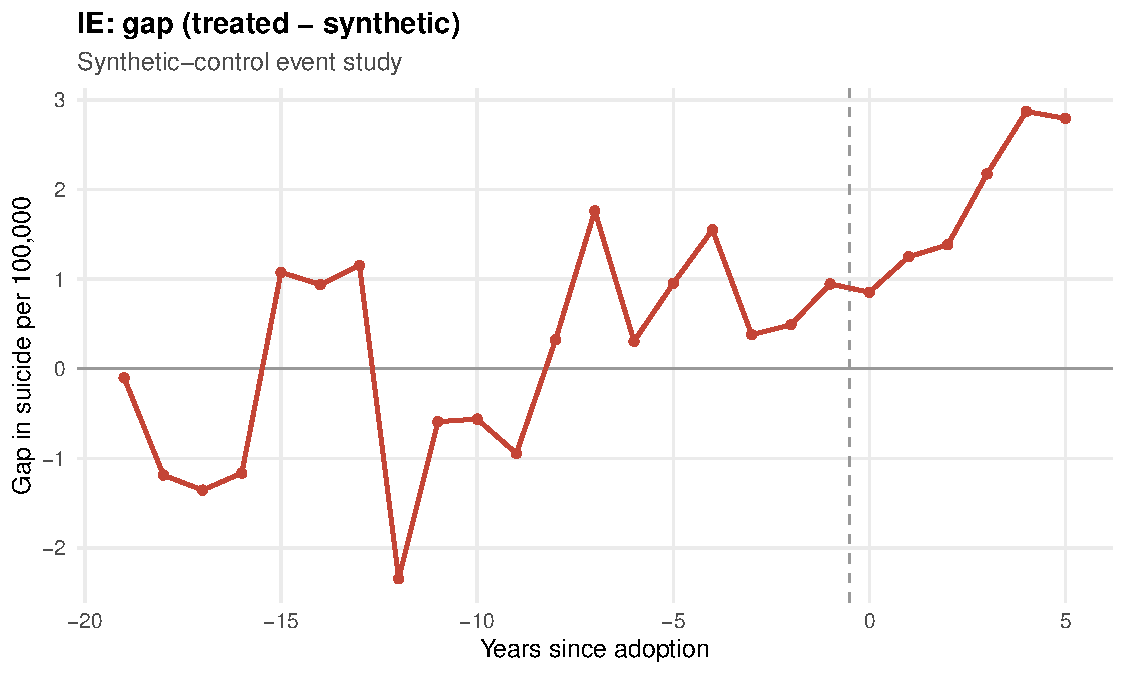
\includegraphics[width=0.49\textwidth]{fig_scm_gap_IE.pdf}\\[2pt]
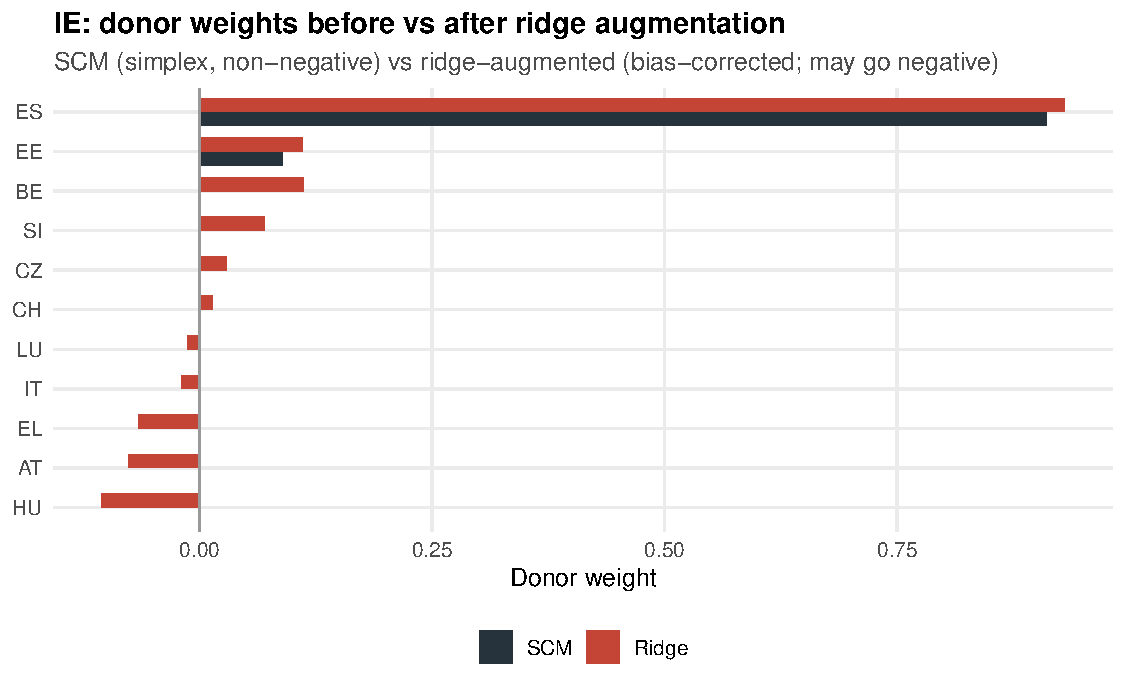
\includegraphics[width=0.49\textwidth]{fig_scm_weights_IE.pdf}\hfill
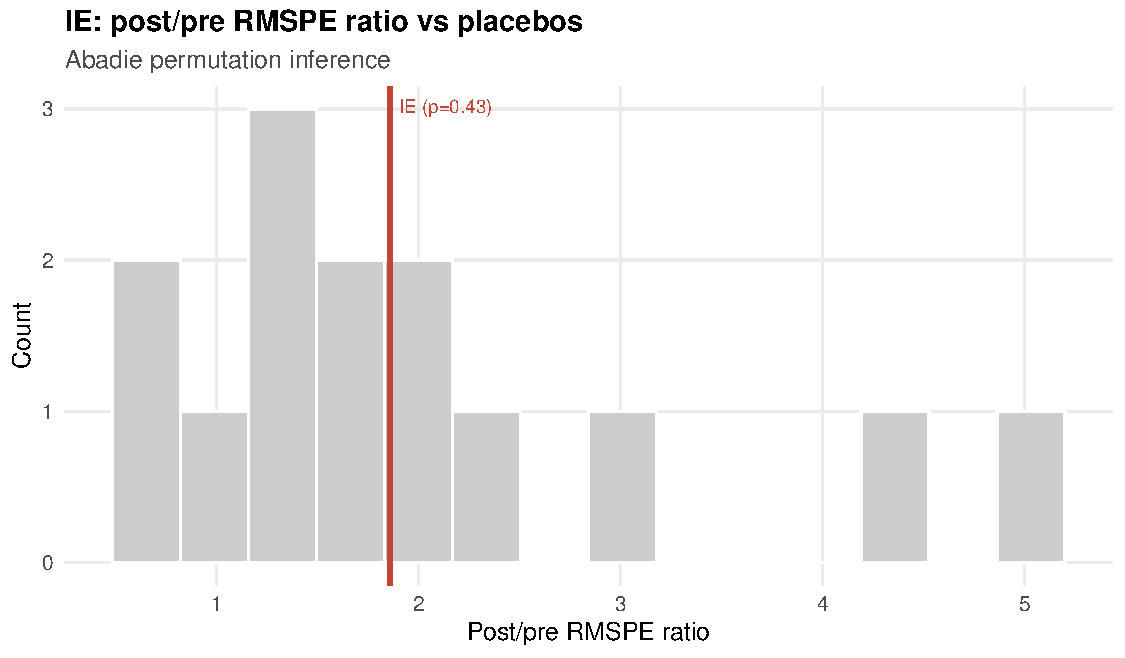
\includegraphics[width=0.49\textwidth]{fig_scm_rmspe_IE.pdf}
\caption{Ireland. Fit, gap, donor weights (before/after ridge), and permutation.}
\end{figure}

\clearpage
\singlespacing
\bibliography{references}

\end{document}
